\documentclass[11pt]{article}

% This is a package for drawing figures
% it is a part of standard latex 2e distribution
\usepackage{tikz}
\usetikzlibrary{positioning,arrows}
\usetikzlibrary{shapes}
\usetikzlibrary{arrows.meta}
\usepackage{fullpage}


\usepackage{palatino}
\RequirePackage{ifthen}
\usepackage{latexsym}
\RequirePackage{amsmath}
\RequirePackage{amsthm}
\RequirePackage{amssymb}
\RequirePackage{xspace}
\RequirePackage{graphics}
\usepackage{xcolor}




\RequirePackage{textcomp}
\usepackage{keyval}
%\usepackage{listings}
\usepackage{xspace}
\usepackage{mathrsfs,paralist, amsmath,amssymb,url,listings,mathrsfs}
%\usepackage{pvs}
%\usepackage{supertabular,alltt,latexsym}
%\usepackage{multicol,multirow,epsfig}
%\usepackage[dvips, usenames]{color}
\usepackage{framed}
\usepackage{lipsum}
%\usepackage[dvipsnames]{color}
\usepackage[linesnumbered]{algorithm2e}
% copyright notice


\definecolor{reddish}{rgb}{1,.8,0.8}
\definecolor{blueish}{rgb}{0.8,.8,1}
\definecolor{greenish}{rgb}{.8,1,0.8}
\definecolor{yellowish}{rgb}{1,1,.20}


\usepackage[pdftex]{hyperref}
\hypersetup{
  pdftitle={Lecture notes for Modeling and Verification of Real-time and Hybrid Systems},
  pdfauthor={Sayan Mitra},
  colorlinks=true,
  citecolor={blue},
  linkcolor = {blue},
  pagecolor={blue},
  backref={true},
  bookmarks=true,
  bookmarksopen=false,
  bookmarksnumbered=true
}

%\newcommand{\remove}[1]{}
\newcommand{\nicole}[1]{\textcolor{red}{#1}}

% \input{prelude1}


\newcommand{\handout}[6]{
  \noindent
  \begin{center}
  \framebox{
    \vbox{
      \hbox to 5.78in { {\bf ECE/CS 584: Embedded and cyberphysical system  verification } \hfill #2 }
      \vspace{4mm}
      \hbox to 5.78in { {\Large \hfill #5  \hfill} }
      \vspace{2mm}
       \hbox to 5.78in { {\Large \hfill #6  \hfill} }
      \vspace{2mm}
      \hbox to 5.78in { {\em #3 \hfill #4} }
    }
  }
  \end{center}
  \vspace*{4mm}
}

\newcommand{\smallheader}[5]{
  \noindent
  \begin{center}
  \framebox{
    \vbox{
      \hbox to 5.78in { {\bf ECE/CS 584: Embedded and cyberphysical system  verification  } \hfill #2 }
      \vspace{2mm}
      \hbox to 5.78in { {\em #3 \hfill #4} }
      \vspace{2mm}
      \hbox to 5.78in { {\em \hfill #5} }
    }
  }
  \end{center}
  \vspace*{4mm}
}

\newcommand{\lecture}[4]{\handout{#1}{#2}{#3}{Scribe: #4}{Lecture #1}}

\newcommand{\homework}[2]{\smallheader{#1}{Fall 2019}{Homework #1}\vspace{5mm}
	{#2}
	}

\newcommand{\solution}[2]{\smallheader{#1}{Fall 2017}{Solutions for Homework #1}{#2}}


\newcommand{\interestingfact}[1]{
	\noindent
	\begin{center}
	\colorbox{yellowish}{
	\parbox{11.5cm}{{\bf Factoid.} #1}
	}
	\end{center}
	\vspace*{4mm}
}
%\definecolor{MyGray}{rgb}{0.96,0.97,0.98}
\makeatletter\newenvironment{color1box}{%
   \begin{lrbox}{\@tempboxa}\begin{minipage}{\columnwidth}}{\end{minipage}\end{lrbox}%
   \colorbox{reddish}{\usebox{\@tempboxa}}
}\makeatother


\makeatletter\newenvironment{color3box}{%
   \begin{lrbox}{\@tempboxa}\begin{minipage}{\columnwidth}}{\end{minipage}\end{lrbox}%
   \colorbox{blueish}{\usebox{\@tempboxa}}
}\makeatother

% 1-inch margins, from fullpage.sty by H.Partl, Version 2, Dec. 15, 1988.
\topmargin 0pt
\advance \topmargin by -\headheight
\advance \topmargin by -\headsep
\textheight 8.9in
\oddsidemargin 0pt
\evensidemargin \oddsidemargin
\marginparwidth 0.5in
\textwidth 6.5in

\parindent 0in
\parskip 1.5ex
%\renewcommand{\baselinestretch}{1.25}

\begin{document}


\smallheader{3 on --- Due on November $14^{th}$}{Fall 2019}{Dawei Sun, daweis2}{Homework 4: Reachability}{Due November $14^{th}$}

\begin{quote}
	{\em Typeset your solutions using \LaTeX\, zip your writeup (.pdf) and code in a single file called \texttt{nedid-584-F19.zip} and upload this file through Compass.}
\end{quote}

\paragraph{Problem 1 (20 points).}
Consider the following decision problem $\mathsf{Mult}$: Given binary
numbers $m,n,$ and $i$, determine if the $i$th bit of the binary
representation of $m\times n$ is $1$. As a language we could define
this as
\[
\mathsf{Mult} = \{(m,n,i)\: |\: \mbox{$i$th bit of $m\times n$ is $1$}\}
\]
Prove that $\mbox{Mult} \in \mbox{L}$ (deterministic log space) by giving the pseudo-code of an algorithm and analyzing its memory requirements in terms of the number
of (additional, non-input) bits it stores.

\paragraph{Solution} Notations: \textbf{len}(m) is the number of digits in m. \textbf{MAX}, \textbf{MIN}, \textbf{mod}, \textbf{floor} are functions. The algorithm is as follows:

\begin{algorithm}[H]
\SetKwInOut{Input}{input}\SetKwInOut{Output}{output}
\SetAlgoLined
\Input{m, n, i}
\Output{Decision}
 $sum = 0$\;
 \For{ri = 1 to i}{
   \For{ni = \textbf{MAX}(1, ri+1-\textbf{len}(m)) to \textbf{MIN}(ri, \textbf{len}(n))}{
     $mi = ri + 1 - ni$\;
     $sum = sum + m[mi]*n[ni]$\;}
   \eIf{ri == i}{\textbf{return} (sum \textbf{mod} 2 == 1)\;}{
     $sum = \textbf{floor}(sum / 2)$\;}}
 \caption{Binary Multiplication}
\end{algorithm}

\textbf{Analysis}: Denote $N$ as the number of digits in $m$ and $n$, i.e. $N = \textbf{len}(m) + \textbf{len}(n)$. Next, we analyze the size of every intermediate variable. Clearly, $ri \leq i \leq N+1$, and thus size of $ri$ is $O(log(N))$. For $mi$ and $ni$ the analysis is similar. Next, we analyze the maximal value of $sum$. We claim that $sum < 2N$ and use induction to prove that. First, when $ri=0$, $sum < 2N$ clearly holds. If $sum < 2N$ holds when $ri=k-1$, then after Line 10 is executed we have $sum < N$. Because during the execution of Line 3-6 the increament of $sum$ is at most $N$, we have $sum<2N$ holds when $ri=k$. Therefore, $sum < 2N$ always holds and thus we know the size of $sum$ is $O(log(N))$.

\paragraph{Problem 2. (10 points)}
Construct the region automaton corresponding to the following timed automaton.

\begin{figure}[h!]
	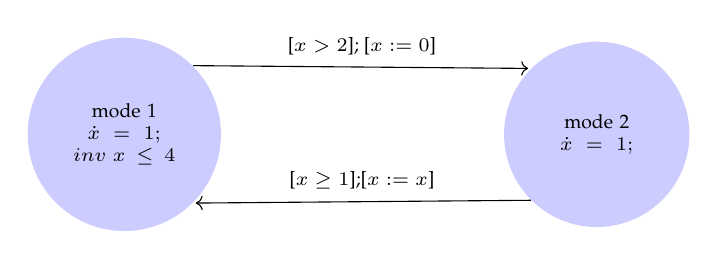
\begin{tikzpicture}
	\tikzstyle{every node}=[font=\scriptsize, circle, fill=blue!20, font=\scriptsize, minimum size = 1.6cm]
	\draw (-3,3) node (oneo) [align=center, text width=2cm]{mode 1 \\$ \dot{x} = 1;$ \\$ inv \ x \leq 4$};
	\draw (3,3) node (two) [align=center, text width=2cm]{mode 2 \\$ \dot{x} = 1;$};

%	\draw (-3,-3) node (p3) {$\dot{x} = -3; \dot{y} =-3$};
%	\draw (3,-3) node (p4) {$\dot{x} = -3; \dot{y}= 2$};
	\tikzstyle{every node}=[font=\scriptsize,fill=none]
	\draw [ shorten >=1pt,->] (oneo.north east) to  node[above=1pt] {[$x > 2$]; [$x:=0$]} (two.north west);
	\draw [ shorten >=1pt,->] (two.south west) to  node[above=1pt] {[$x\geq 1$];[$x := x$]} (oneo.south east);
	\end{tikzpicture}
\end{figure}

\paragraph{Solution} Region automaton:

\begin{figure}[h!]
	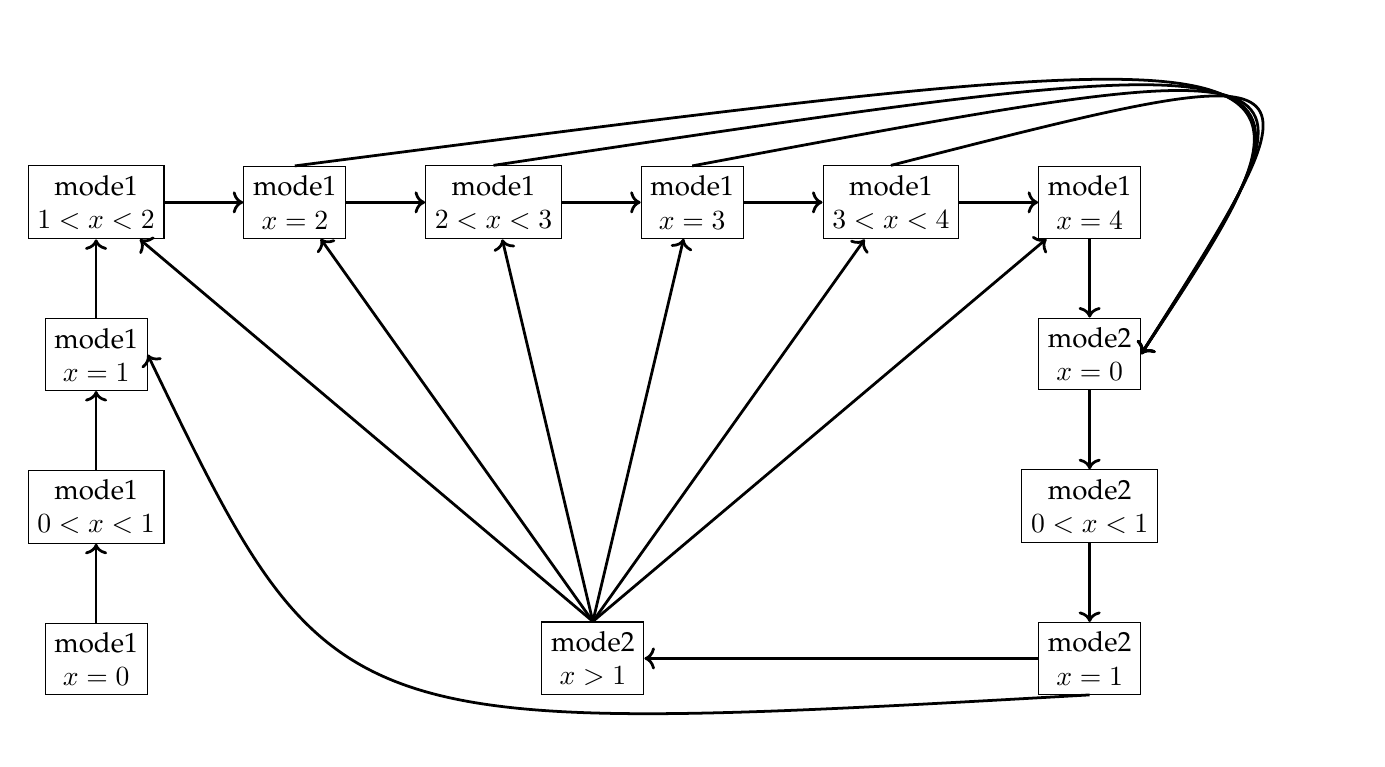
\begin{tikzpicture}
	\tikzstyle{every node}=[align=center, draw, rectangle]
  % \draw [step=1.0,blue, very thick] (0,0) grid (15,10);
  \node [] (n1) {mode1\\$x=0$};
  \node [above = of n1] (n2) {mode1\\$0<x<1$};
  \node [above = of n2] (n3) {mode1\\$x=1$};
  \node [above = of n3] (n4) {mode1\\$1<x<2$};
  \node [right = of n4] (n5) {mode1\\$x=2$};
  \node [right = of n5] (n6) {mode1\\$2<x<3$};
  \node [right = of n6] (n7) {mode1\\$x=3$};
  \node [right = of n7] (n8) {mode1\\$3<x<4$};
  \node [right = of n8] (n9) {mode1\\$x=4$};
  \node [below = of n9] (n10) {mode2\\$x=0$};
  \node [below = of n10] (n11) {mode2\\$0<x<1$};
  \node [below = of n11] (n12) {mode2\\$x=1$};
  \node [left = 5cm of n12] (n13) {mode2\\$x>1$};

  \draw [->, line width=1pt] (n1) -- (n2);
  \draw [->, line width=1pt] (n2) -- (n3);
  \draw [->, line width=1pt] (n3) -- (n4);
  \draw [->, line width=1pt] (n4) -- (n5);
  \draw [->, line width=1pt] (n5) -- (n6);
  \draw [->, line width=1pt] (n6) -- (n7);
  \draw [->, line width=1pt] (n7) -- (n8);
  \draw [->, line width=1pt] (n8) -- (n9);
  \draw [->, line width=1pt] (n9) -- (n10);
  \draw [->, line width=1pt] (n10) -- (n11);
  \draw [->, line width=1pt] (n11) -- (n12);
  \draw [->, line width=1pt] (n12) -- (n13);
  \draw [->, line width=1pt] (n5.north) .. controls (16,8) .. (n10.east);
  \draw [->, line width=1pt] (n6.north) .. controls (15.9,7.9) .. (n10.east);
  \draw [->, line width=1pt] (n7.north) .. controls (15.8,7.8) .. (n10.east);
  \draw [->, line width=1pt] (n8.north) .. controls (15.7,7.7) .. (n10.east);
  \draw [->, line width=1pt] (n12.south) .. controls (3,-1) .. (n3.east);
  \draw [->, line width=1pt] (n13.north) -- (n4);
  \draw [->, line width=1pt] (n13.north) -- (n5);
  \draw [->, line width=1pt] (n13.north) -- (n6);
  \draw [->, line width=1pt] (n13.north) -- (n7);
  \draw [->, line width=1pt] (n13.north) -- (n8);
  \draw [->, line width=1pt] (n13.north) -- (n9);
	\end{tikzpicture}
\end{figure}


\paragraph{Problem 3 (10 points).}
(a) Convert the rectangular initialized hybrid automaton of Figure~\ref{fig:irha}
to a timed automaton (clocks may be initialized to constant intervals).
The first expression on the arrows are the preconditions/guards and the second expresssion
is the effect or the reset function. No reset implies that the state variables are not reset.

(b) Plot an execution of the original hybrid automaton and the corresponding execution
of the timed automaton.
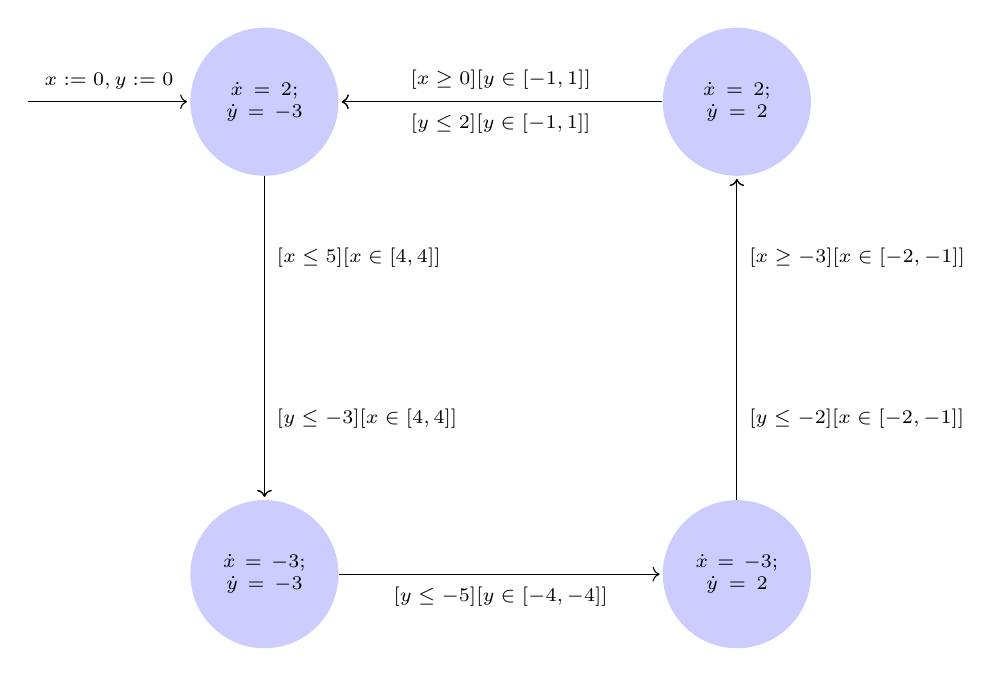
\begin{tikzpicture}
	\tikzstyle{every node}=[font=\scriptsize, circle, fill=blue!20, font=\scriptsize, minimum size = 1.6cm]
	\draw (-3,3) node (p1) [align=center, text width=1.5cm]{$\dot{x} = 2;$\\$\dot{y} =-3$};
	\draw (3,3) node (p2) [align=center, text width=1.5cm]{$\dot{x} = 2;$\\$ \dot{y} =2$};
	\draw (-3,-3) node (p3) [align=center, text width=1.5cm]{$\dot{x} = -3;$\\$ \dot{y} =-3$};
	\draw (3,-3) node (p4) [align=center, text width=1.5cm]{$\dot{x} = -3;$\\$ \dot{y}= 2$};
	\tikzstyle{every node}=[font=\scriptsize,fill=none]
	\draw [ shorten >=1pt,->] (-6,3) to  node[above=1pt] {$x:=0, y:=0$} (p1);
	\draw [ shorten >=1pt,->] (p2) to  node[above=1pt] {$[x\geq 0][y \in [-1,1]]$} (p1);
	\draw [ shorten >=1pt,->] (p2) to  node[below=1pt] {$[y\leq 2][y \in [-1,1]]$} (p1);
	\draw [ shorten >=1pt,->] (p1) to  node[right=1pt, near start] {$[x\leq 5][x \in [4,4]]$} (p3);
	\draw [ shorten >=1pt,->] (p1) to  node[right=1pt, near end] {$[y\leq -3][x \in [4,4]]$} (p3);
	\draw [ shorten >=1pt,->] (p4) to  node[right=1pt, near start] {$[y\leq -2][x \in [-2,-1]]$} (p2);
	\draw [ shorten >=1pt,->] (p4) to  node[right=1pt, near end] {$[x\geq -3][x \in [-2,-1]]$} (p2);
	\draw [ shorten >=1pt,->] (p3) to  node[below=1pt] {$[y\leq -5][y \in [-4,-4]]$} (p4);
\end{tikzpicture}

\paragraph{Solution}
\begin{itemize}
\item

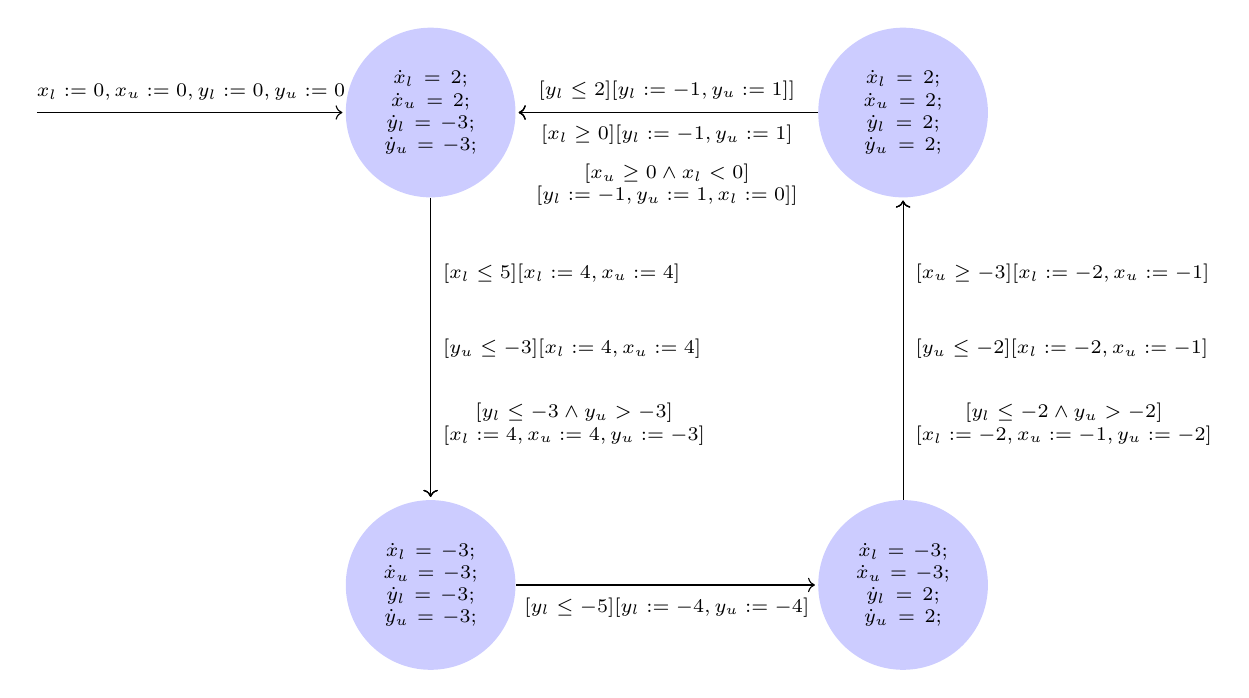
\begin{tikzpicture}
	\tikzstyle{every node}=[font=\scriptsize, circle, fill=blue!20, font=\scriptsize, minimum size = 1.6cm]
	\draw (-3,3) node (p1) [align=center, text width=1.5cm]{$\dot{x}_l = 2;$\\$\dot{x}_u = 2;$\\$\dot{y}_l =-3;$\\$\dot{y}_u =-3;$};
	\draw (3,3) node (p2) [align=center, text width=1.5cm]{$\dot{x}_l = 2;$\\$\dot{x}_u = 2;$\\$\dot{y}_l =2;$\\$\dot{y}_u =2;$};
	\draw (-3,-3) node (p3) [align=center, text width=1.5cm]{$\dot{x}_l = -3;$\\$\dot{x}_u = -3;$\\$\dot{y}_l =-3;$\\$\dot{y}_u =-3;$};
	\draw (3,-3) node (p4) [align=center, text width=1.5cm]{$\dot{x}_l = -3;$\\$\dot{x}_u = -3;$\\$\dot{y}_l =2;$\\$\dot{y}_u =2;$};
	\tikzstyle{every node}=[font=\scriptsize,fill=none]
	\draw [ shorten >=1pt,->] (-8,3) to  node[above=1pt] {$x_l:=0, x_u:=0, y_l:=0, y_u:=0$} (p1);
  \draw [ shorten >=1pt,->] (p2) to  node[above=1pt] {$[y_l \leq 2][y_l:=-1, y_u:=1]]$} (p1);
  \draw [ shorten >=1pt,->] (p2) to  node[below=1pt] {$[x_l \geq 0][y_l:=-1, y_u:=1]$} (p1);
  \draw [ shorten >=1pt,->] (p2) to  node[below=15pt, align=center] {$[x_u \geq 0 \wedge x_l < 0]$\\$[y_l:=-1, y_u:=1, x_l:=0]]$} (p1);
	\draw [ shorten >=1pt,->] (p1) to  node[right=1pt, near start] {$[x_l \leq 5][x_l:=4, x_u:=4]$} (p3);
  \draw [ shorten >=1pt,->] (p1) to  node[right=1pt] {$[y_u \leq -3][x_l:=4, x_u:=4]$} (p3);
	\draw [ shorten >=1pt,->] (p1) to  node[right=1pt, near end, align=center] {$[y_l \leq -3 \wedge y_u > -3]$\\$[x_l:=4, x_u:=4, y_u:=-3]$} (p3);
  \draw [ shorten >=1pt,->] (p4) to  node[right=1pt, near start, align=center] {$[y_l \leq -2 \wedge y_u > -2]$\\$[x_l:=-2, x_u:=-1, y_u:=-2]$} (p2);
	\draw [ shorten >=1pt,->] (p4) to  node[right=1pt] {$[y_u\leq -2][x_l:=-2, x_u:=-1]$} (p2);
	\draw [ shorten >=1pt,->] (p4) to  node[right=1pt, near end] {$[x_u\geq -3][x_l:=-2, x_u:=-1]$} (p2);
  \draw [ shorten >=1pt,->] (p3) to  node[below=1pt] {$[y_l \leq -5][y_l:=-4, y_u:=-4]$} (p4);
\end{tikzpicture}

\item

\begin{figure}[h]
  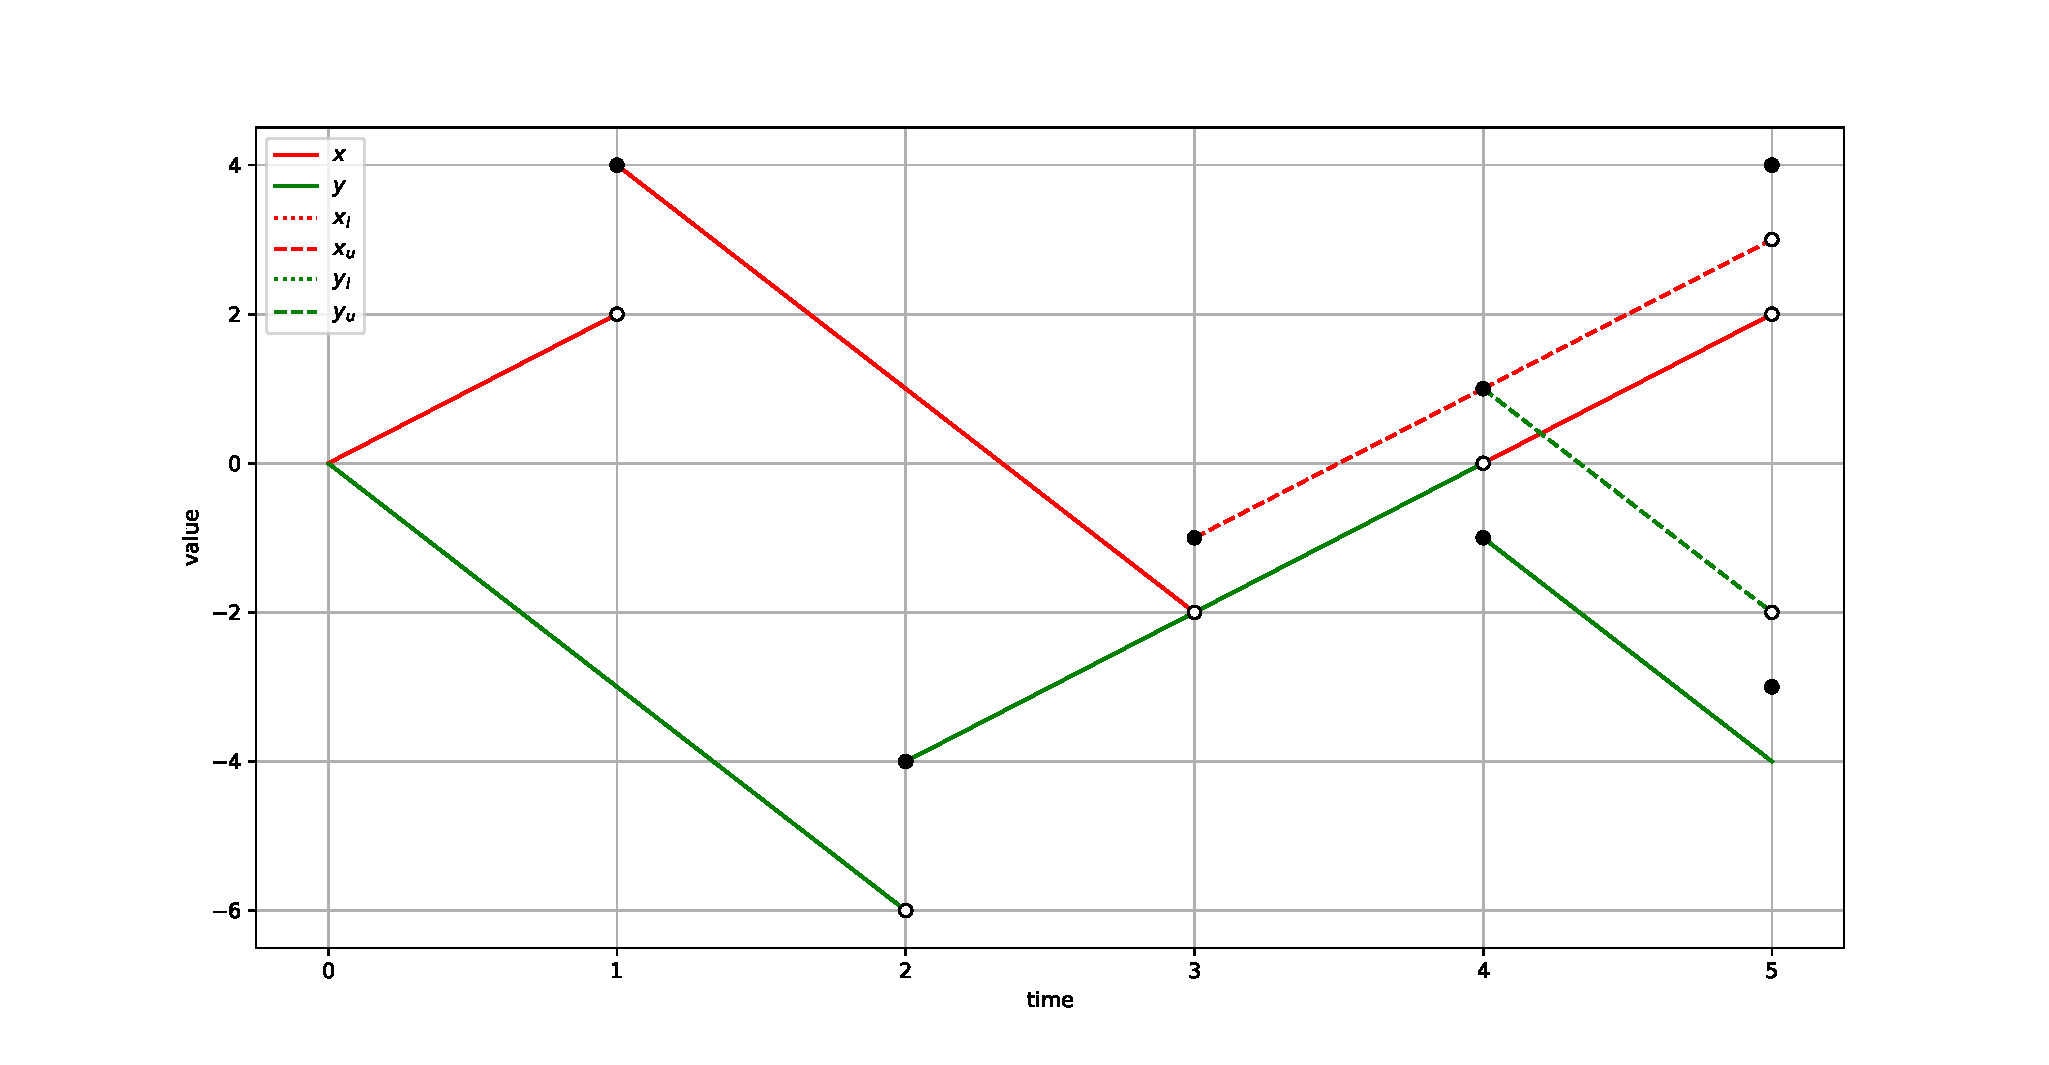
\includegraphics[width=\linewidth]{plot}
  \caption{plot of execution}
  \label{}
\end{figure}
\end{itemize}

\paragraph{Problem 4 (20 points).}
Consider a system with two leaky tanks $T_1$ and $T_2$ and an inflow pipe $P$
which can feed to either of the tanks. The inflow rate from $P$, when on, is $f_{in}$, and the outflow
rates from the tanks (independent of any inflow) are $f_1$ and $f_2$. These rates are measured in terms
of the rate of drop (and rise) of the water levels in the tanks. The controller for $P$ is designed such that
within $\delta$ time of the level in tank $i$ dropping below $h_i$, the pipe $P$ is turned to feed $T_i$.
\begin{enumerate}[(a)]
	\item Model the system as a hybrid automaton. Show the circle-arrow representation.
	\item Under what conditions does the model display Zeno behavior ?
	\item Under what conditions can it be guaranteed that neither tank becomes empty? Prove it.
\end{enumerate}

\paragraph{Solution}

\begin{enumerate}[(a)]
	\item Variables: $\ell_1$ the level of tank 1, $\ell_2$ the level of tank 2, $t$ a timer. Constants: $\ell_{10}, \ell_{20}$ the initial value of $\ell_1, \ell_2$.

  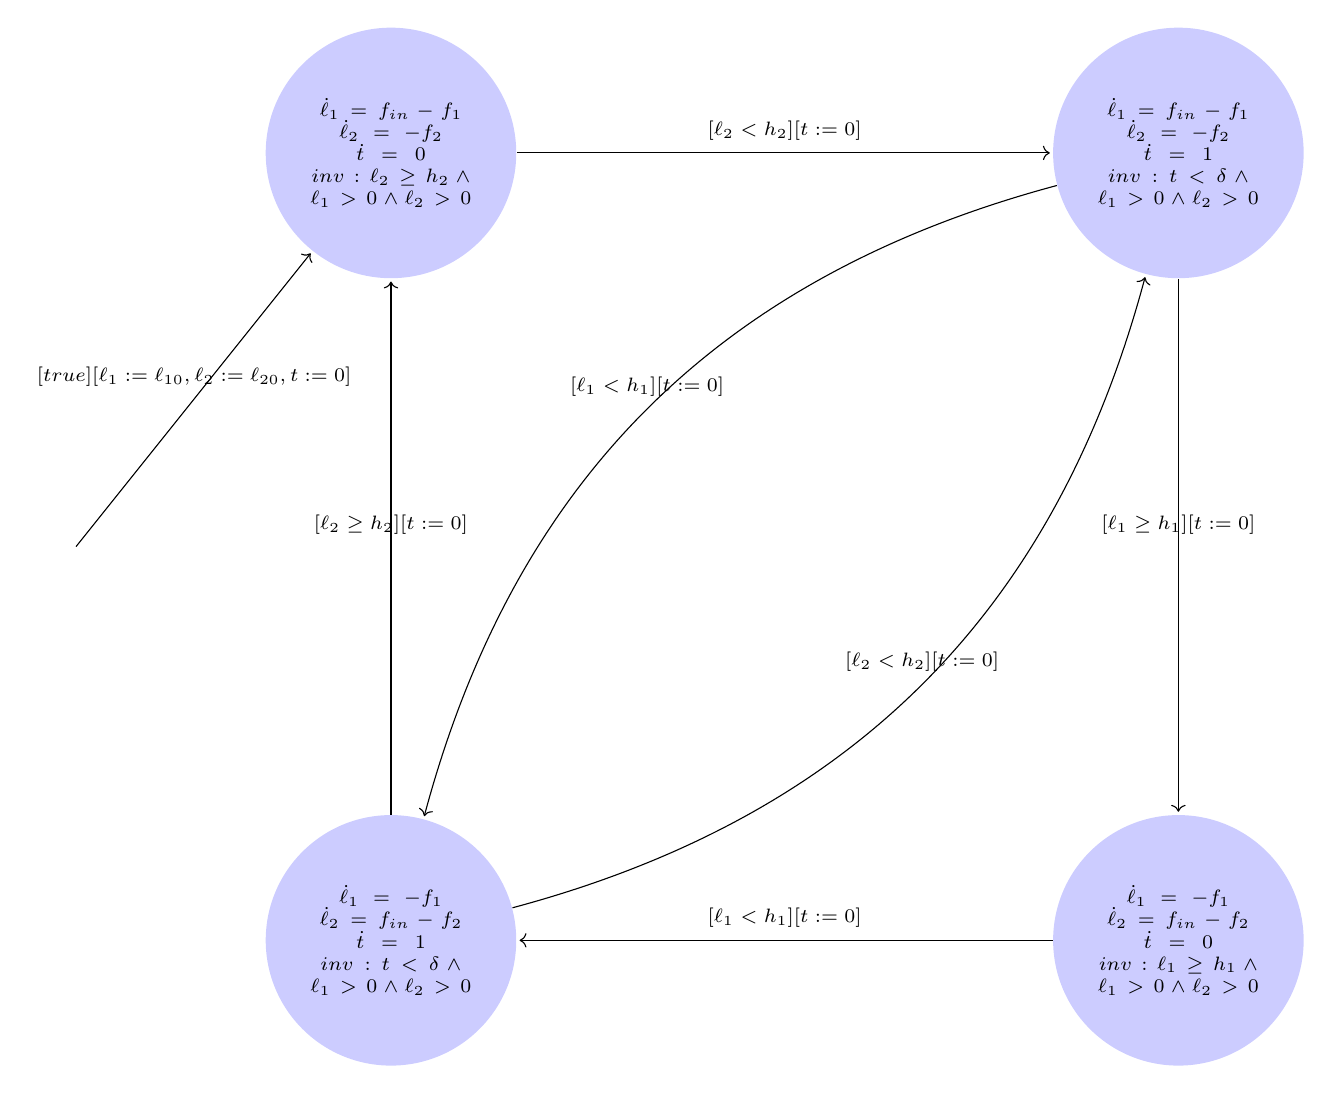
\begin{tikzpicture}
  	\tikzstyle{every node}=[font=\scriptsize, circle, fill=blue!20, font=\scriptsize, minimum size = 2.5cm]
  	\draw (-5,5) node (filling_1_safe) [align=center, text width=2.5cm]{$\dot{\ell}_1 = f_{in} - f_1$\\$\dot{\ell}_2 = -f_2$\\$\dot{t} = 0$\\$inv: \ell_2 \geq h_2 \wedge \ell_1>0 \wedge \ell_2>0$};
  	\draw (5,5) node (filling_1_unsafe) [align=center, text width=2.5cm]{$\dot{\ell}_1 = f_{in} - f_1$\\$\dot{\ell}_2 = -f_2$\\$\dot{t} = 1$\\$inv: t < \delta \wedge \ell_1>0 \wedge \ell_2>0$};
  	\draw (5,-5) node (filling_2_safe) [align=center, text width=2.5cm]{$\dot{\ell}_1 = -f_1$\\$\dot{\ell}_2 = f_{in} - f_2$\\$\dot{t} = 0$\\$inv: \ell_1 \geq h_1 \wedge \ell_1>0 \wedge \ell_2>0$};
  	\draw (-5,-5) node (filling_2_unsafe) [align=center, text width=2.5cm]{$\dot{\ell}_1 = -f_1$\\$\dot{\ell}_2 = f_{in} - f_2$\\$\dot{t} = 1$\\$inv: t < \delta \wedge \ell_1>0 \wedge \ell_2>0$};
  	\tikzstyle{every node}=[font=\scriptsize,fill=none]
  	\draw [ shorten >=1pt,->] (-9,0) to  node[above=1pt] {$[true][\ell_1:=\ell_{10}, \ell_2:=\ell_{20}, t:=0]$} (filling_1_safe);
    \draw [ shorten >=1pt,->] (filling_1_safe) to  node[above=1pt] {$[\ell_2 < h_2][t:=0]$} (filling_1_unsafe);
    \draw [ shorten >=1pt,->] (filling_1_unsafe) to node[above=1pt] {$[\ell_1 \geq h_1][t:=0]$} (filling_2_safe);
  	\draw [ shorten >=1pt,->] (filling_1_unsafe) to [bend right] node[above=1pt] {$[\ell_1 < h_1][t:=0]$} (filling_2_unsafe);
    \draw [ shorten >=1pt,->] (filling_2_safe) to  node[above=1pt] {$[\ell_1 < h_1][t:=0]$} (filling_2_unsafe);
    \draw [ shorten >=1pt,->] (filling_2_unsafe) to  node[above=1pt] {$[\ell_2 \geq h_2][t:=0]$} (filling_1_safe);
    \draw [ shorten >=1pt,->] (filling_2_unsafe) to [bend right] node[above=1pt] {$[\ell_2 < h_2][t:=0]$} (filling_1_unsafe);
  \end{tikzpicture}

	\item When $\ell_1 < h1 \wedge \ell_2 < h2$, the model may display Zeno behavior (via the two bend arrows in the firure)?
	\item A sufficient condition is ``$\ell_{10} > h_1 > \delta f_1, \ell_{20} > h_2 > \delta f_2, (f_{in} - f_1)(f_{in} - f_2) \geq f_1f_2, f_{in}>0$".

  Proof: Without loss of generality, we assume initially the pipe is filling tank1. When $t = \frac{\ell_{20} - h_2}{f_2}$, the level of tank2 is $h_2$. So, the pipe will transit to tank2 at $t_1 \in [\frac{\ell_{20} - h_2}{f_2}, \frac{\ell_{20} - h_2}{f_2}+\delta]$. Then, when $t = t_1 + \frac{\ell_{10} + (f_{in}-f_1)t_1 - h_1}{f_1} > t_1 + \frac{(f_{in}-f_1)t_1}{f_1}$, the level of tank1 will be $h_1$. So between $[t_1, t_1 + \frac{(f_{in}-f_1)t_1}{f_1}]$, the pipe is filling tank2. It is easy to check that between $[0, t_1 + \frac{(f_{in}-f_1)t_1}{f_1}]$, neither tank gets empty because $h_1 > \delta f_1, h_2 > \delta f_2$. At time $t_1 + \frac{(f_{in}-f_1)t_1}{f_1}$, $\ell_1 = \ell_{10} + (f_{in}-f_1)t_1 - f_1 \frac{(f_{in}-f_1)t_1}{f_1} = \ell_{10}$, and $\ell_2 = \ell_{20} - f_2 t_1 + (f_{in}-f_2)\frac{(f_{in}-f_1)t_1}{f_1} \geq \ell_{20}$ because $(f_{in} - f_1)(f_{in} - f_2) \geq f_1f_2$. Ath this point, $\ell_1$ and $\ell_2$ satisfies the condition again. So by the inductive theorem, we know this condition is an invariant, and thus neither tank will be empty.
\end{enumerate}


\paragraph{Problem 5 (40 points).}
Implement a basic reachability analysis algorithm for the billiards problem (from homework 2). To fix notations,  let the state of the $i$th ball in the billiard table be  $(x_i, y_i, v_i, u_i) \in \reals^4$, where $v_i$ and $u_i$   are the velocities along $x$ and $y$ directions. Let $a, b > 0$ be the length and the width of the table.  The algorithm should  take as input:
\begin{enumerate}
\item The number $n > 0$ of balls.
\item The (uncertain) initial position intervals $X_i \subsetneq [0,a], Y_i \subsetneq [0,b]$, for each $i \in [n]$, where $X_i$ is the uncertainty in initial $x$ position and $y$ is the uncertainty in initial $y$ position of the $i$th ball.
\item The (fixed) initial velocities $v_{0,i}$ and $u_{0,i}$.
\item A set of unsafe locations specified as squares for one or more of the balls, just like the specification of the initial states.
\item A time bound $T$.
\end{enumerate}
The output of the algorithm should be:
\begin{enumerate}
	\item The set of reachable states of the balls starting from the specified initial positions, up to the time bound $T$.
	\item A safety check answer that either shows that (a) the ball(s) does not reach the specified unsafe set, or (b) finds a particular initial configuration which makes the ball reach the unsafe set.
\end{enumerate}
For simplicity, use rectangles (or hyperrectangles) to represent the reachable states of each ball.
%

Your reach set computer should propagate the uncertainties in the position correctly as the balls {\em bounce\/} on the walls of the billiard table. Assume that corners belong to one of the sides. However, note that because of the uncertainty in initial position, you will have to consider multiple bounce transitions that may occur for all the states described by a rectangle.

You may ignore ball-ball collisions. Bonus points for handling collisions properly with appropriate explanations. Note that if you ignore collisions, then you can compute the reachset of each ball independently.

You may use one of the reachability analysis tools like C2E2~\cite{FanQM0D16}, Flow*~\cite{flow}, CORA~\cite{CORA16}, or SpaceEx~\cite{Spaceex} {\em at your own risk\/}. That is, we will not be able to provide detailed consulting or bugfixes.

This problem will be graded based on a 10 minute demo where you will have to run the program and answer some questions.

\paragraph{Solution}
Some key observations:
\begin{itemize}
  \item The interactions between the walls and the balls are linear. Starting from a convex initial set, the reachbale set at time $t$ is also a convex set and the vertices corresponds to the vertices of the intial set.
\end{itemize}

\bibliography{sayan1}
	\bibliographystyle{plain}
\end{document}
